\section{Разработка архитектуры наземной станции}

Аппаратная часть наземной станции изначально состояла из:
\begin{itemize}
	\item компьютера;
	\item передающего модуля радиоуправления;
	\item видеоприемника;
	\item устройства приема-передачи телеметрии.
\end{itemize}
% дописать переписать всю кашу, время
Планировалось, что наземная станция должна обмениваться телеметрией с квадрокоптером с помощью радиомодулей, получать видеопоток с квадрокоптера через видеоприемник и отправлять управляющий сигнал в виде команд MAVROS с помощью телеметрийных модулей. 
% в данной парадигме структура наземной станции следующая:
К компьютеру по UART порту подключался модуль радиоуправления и устройство приема-передачи телеметрии. Через USB порт подключался видеоприемник. Настраивался видеоприемник на диапазон частот, соответствующий частотам видеопередатчика квадрокоптера, и далее следовала настройка программной части.
Чем больше бод -- рейт подключенных модулей и меньше задержка сигнала, тем быстрее осуществляется выполнение команд. Учитывая эти факторы, выбираются устройства телеметрии и видеоприемник.
% дописать
К компьютеру по UART порту подключался модуль радиоуправления и устройство приема-передачи телеметрии. Через USB порт подключался видеоприемник (рисунок \ref{fig:ns}). Настраивался видеоприемник на диапазон частот, соответствующий частотам видеопередатчика квадрокоптера, и далее следовала настройка программной части.
\begin{figure}[H]
	\centering
	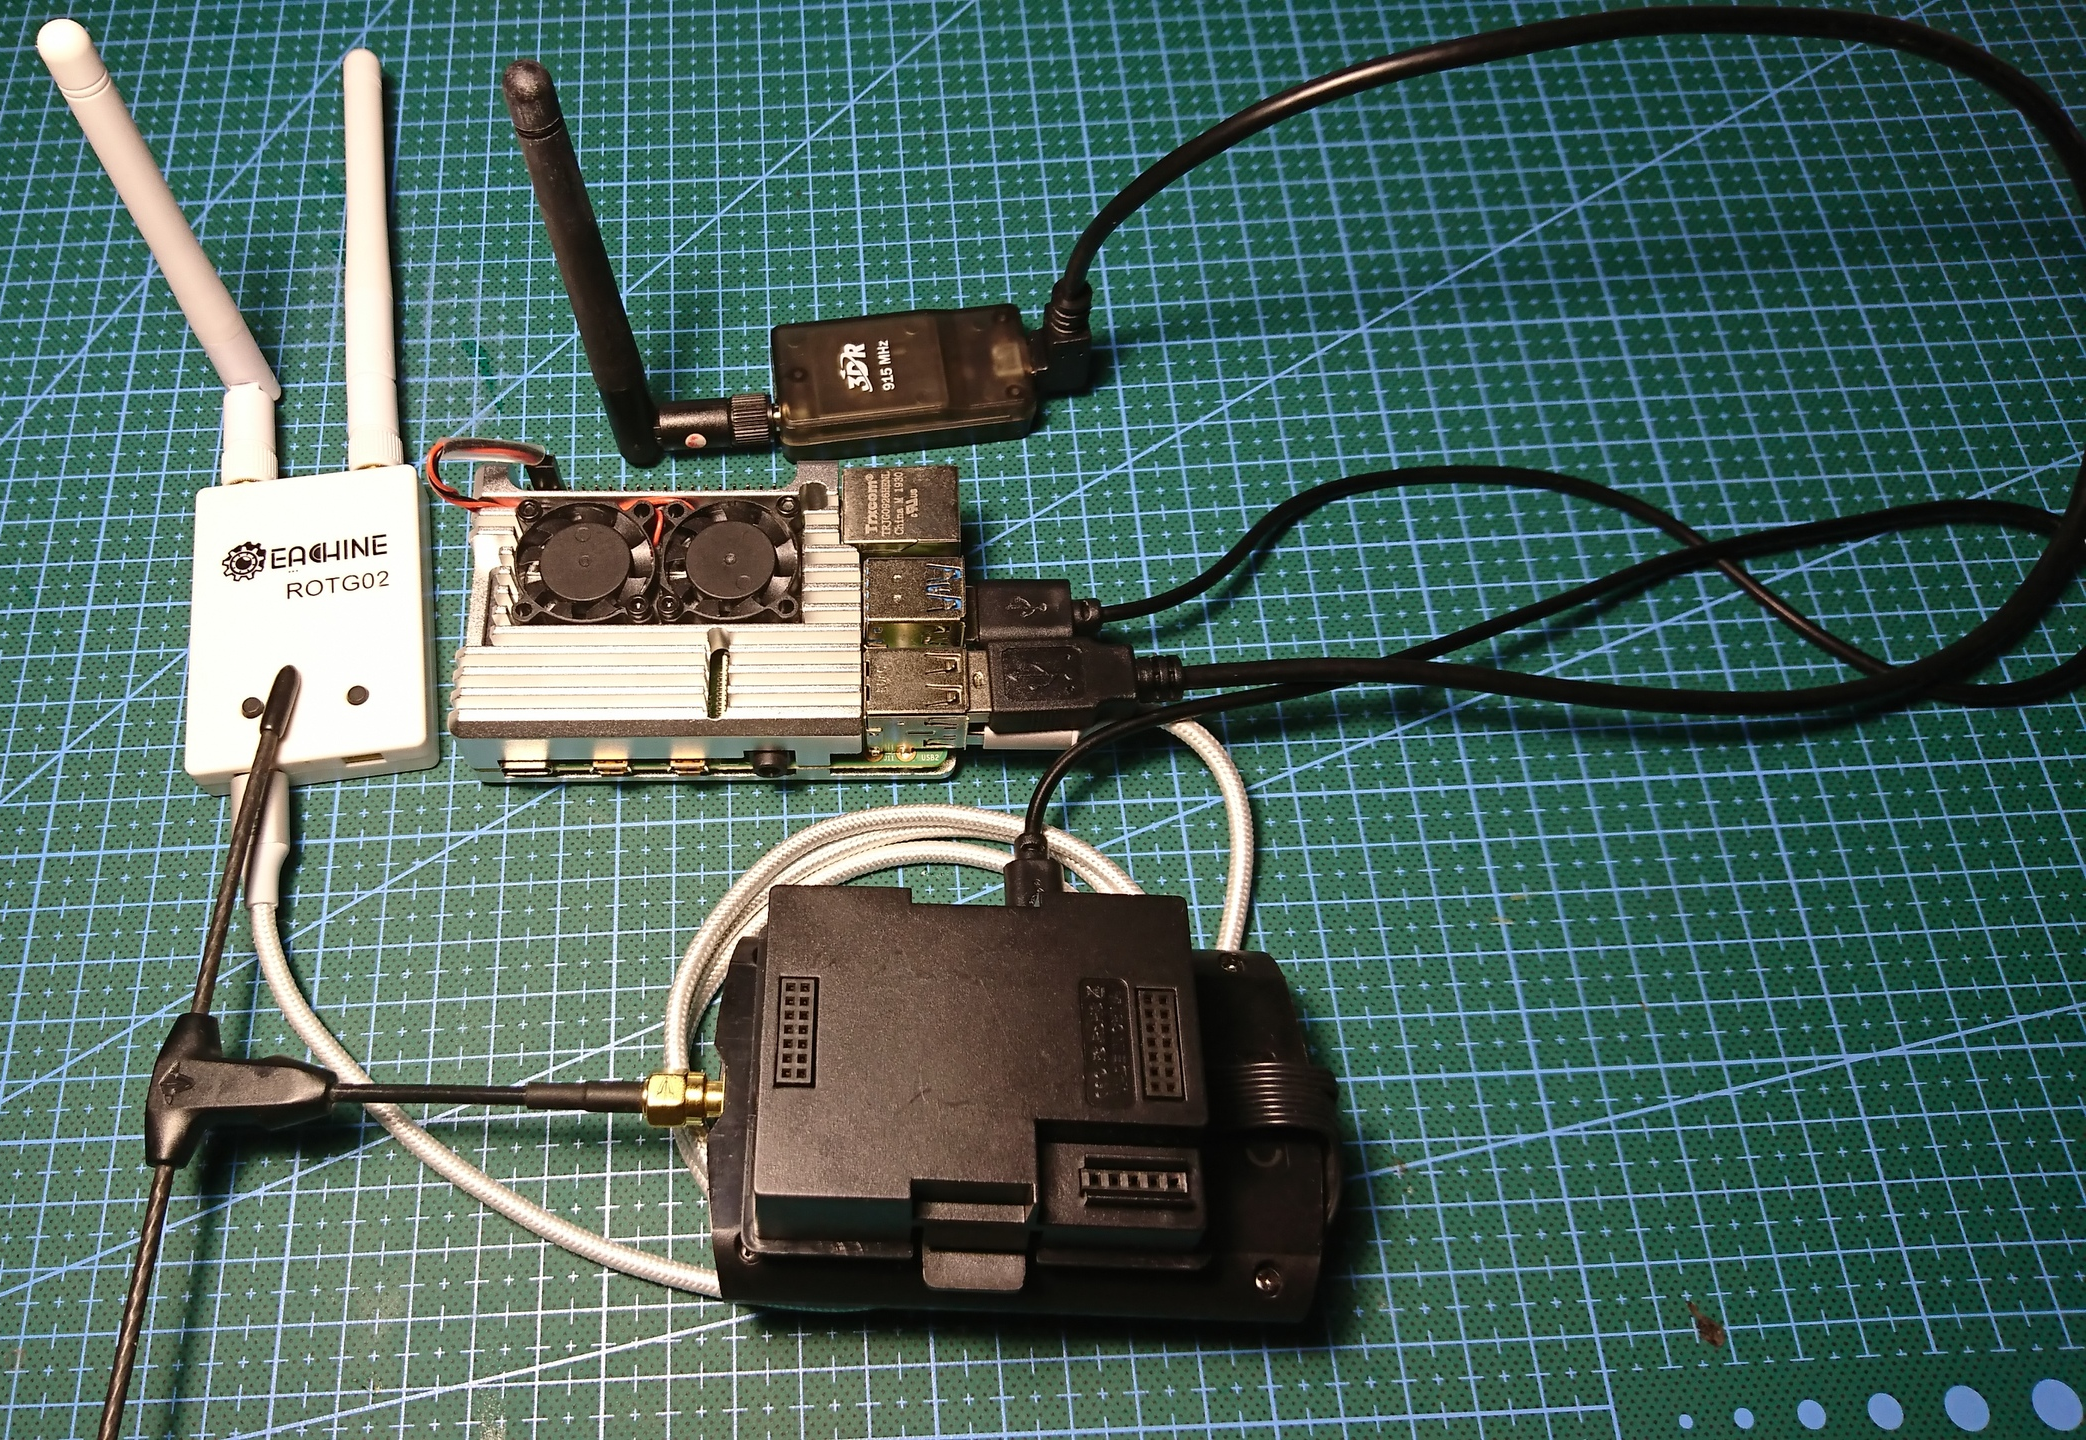
\includegraphics[width=0.5\linewidth]{./pics/qgc}
	\caption{Первый экспериментальный образец наземной станции
	}
	\label{fig:ns} % эта метка позволяет ссылаться на рисунок в тексте
\end{figure}

Однако в ходе выполнения научно-исследовательской работы \cite{nir3} был выявлен более оптимальный способ обмена информации -- по wifi-соединению. Такой способ позволяет уменьшить задержку, количество компонентов, а значит и стоимость комплекта, и использовать персональный компьютер в качестве наземной станции. 
 % дописать преимущества такого решения
%куда необходимо поставить несколько программных решений и настроить взаимодействие между ними.

Таким образом, наземная станция представляет собой компьютер, находящийся в одной подсети с RPi дрона.
ПО наземной станции представляет собой совокупность таких решений как:
\begin{itemize}
	\item операционная система семейства ubuntu версии 16 / 18 на базе ядра linux версии 5.3.0*;
	\item пакетов ros-*;
	\item mavros;
	\item gstreamer;
	\item aruco\_gridboard в связке с gscam.
\end{itemize}
%дописать как это работает. у меня теперь малина регистрирует изображение с камеры, передает на наземную станцию..

\subsection{Конфигурация наземной станции}

\subsubsection{Настройка MAVROS}

Первым делом производится запуск ROS среды посредством roscore. Далее настраиваются конфигурационные файлы.

Для получения телеметрии полетного контроллера необходимо в файле /opt/ros/melodic/share/mavros/launch/px4.launch поменять параметр fcu\_url, указав нужный адрес и порт. Параметр gcs\_url задает адрес для проксирования MAVLink сообщений под нужды qgroundcontrol (листинг \ref{lst:9}):
\begin{Program}[H]
	\caption{Измененные параметры в launch файле mavros} \label{lst:9}
	\begin{MyCode}
	<arg name="fcu_url" default="tcp://192.168.1.148:2000?ids=1,240"/>   
	<arg name="gcs_url" default="udp://@127.0.0.1:14555"/>
	\end{MyCode}
\end{Program}

\subsubsection{Подготовка инструментов для получения и обработки видеопотока}
Для получения трансляции и публикации топиков с изображением с камеры используется пакет gscam. Он собирается из репозитория \url{https://github.com/ros-drivers/gscam} командами, представленными в листинге \ref{lst:10}:
\begin{Program}[H]
	\caption{Сборка gscam} \label{lst:10}
	\begin{MyCode}
	$ git clone https://github.com/ros-drivers/gscam
	$ cd gscam
	$ cmake -DGSTREAMER_VERSION_1_x=On
	$ сmake install
	\end{MyCode}
\end{Program}

Распознавание карты aruco маркеров на изображении, получаемом из топиков gscam, и публикацию полученных координат в топик /vision/pose производит пакет aruco\_gridboard. Команды для сборки этого пакета представлены в листинге \ref{lst:11}:
\begin{Program}[H]
	\caption{Сборка aruco\_gridboard} \label{lst:11}
	\begin{MyCode}	
	$ cd ~/catkin_ws/src
	$ git clone https://github.com/anbello/aruco_gridboard.git
	$ cd ..
	$ catkin_make
	$ source devel/setup.bash
	$ catkin_make --only-pkg-with-deps aruco_gridboard
	\end{MyCode}
\end{Program}

Проделанных шагов достаточно, чтобы на наземной станции отобразить положение дрона относительно карты маркеров.
